\chapter{Memory Game}
\label{memory_game}

%- Bei dem zum simulieren des glare effects genutzen spiel handelt es sich um Memory (matching pairs game).  Das spiel enntält diverse Spielmodi, in welchen verschiedene memory oder visual obstacles existieren. Beispielsweise kann das Hinderniss einer allgemeinen sehschwäche, der rot grün schwäche oder auch, was für diese arbeit von bedeutung ist, das Blenden des Bildschirms durch einfallende sonnenstrahlung simuliert werden. Ebenso bietet das spiel mehrere möglichkeiten der adaption, wie besipielsweise das erneute vorzeigen der karten aus dem letzten zug oder die zuweisung von buchstaben zu kartenpaaren welche beim umdrehen einer karte ausgesproche werden. Erstere stellt einen gedächtnis assistenten für memory obstacles da während die zweite im fall visueller Hindernisse eine neue art erzeugt anhand der sich die spieler orientieren können. Dies sind nicht alle funktionalitäten die das spiel bietet, aber da nur bestimmte von relevanz für diese arbeit sind werden nicht alle erläutert. Für diese arbeit sind von besonderer bedeutung der modus ohne hindernisse und der modus mit glare effect. 

The game used for the data collection is a matching pairs game written in Kotlin for Android devices. The original version was developed by Rafael Miranda \todo{ref} in the context of a bachelor thesis. Originally, the game consisted of cards picturing animals and was only used to model general poor eyesight. Later is was expanded by adding a coloured card set to also model colour blindness. In the following the current functionalities of the game will be explained, only covering those related to the coloured cards. One game consists of 14 cards and each round consists of two cards being turned face up. If the cards match, they will be removed from the field. Otherwise they are turned face down again. The player wins once all 7 pairs have been discovered. 

The game differentiates between two groups of obstacles: memory obstacles and visual obstacles. Additionally there is a classic mode providing the possibility to play without any obstacles which uses the red-green card set, shown in fig \todo{ref}. The memory obstacle mode consists of the same card set and an additional side task: Every time a card is flipped a random number between 0 ans 10 is called out and the player must add all these numbers. After the final pair was found the sum of all numbers is requested. The game contains modes for two types of visual obstacles: Colour blindness and the glare effect. Colour blindness, more precisely a red-green weakness, is simulated by replacing the red-green card set with a brown shifted card set. The glare effect describes a sczenatio in which a lightsource shines onto the display, reflects from it and makes it more difficult to differnentiate the colours of the cards. This effect can be seen in figure \todo{ref}. 

To help in case of interaction obstacles the game provides multiple ways of assistance. Although they are not relevent for this thesis as only data is used where probants had no assistance, they will be explained briefly. There are two types of assistance: memory and visual assistance. Memory assistance is provided by flipping the cards from the previous turn once two non matching cards are flipped. After a short period of time they are turned face down again. If the game is played with visual assistance, each pair gets assigned a letter that is called out once a card is flipped. This introduces a new way of orientation that does not rely on the sense of sight, but instead on the sense of hearing. There is a game mode for each combination of obstacle (no obstacle, memory obstacle, colour blindness, glare effect) and assistance (no assistance, memory assistance, visual assistance). There where also other assistances implemented such as increasing the size of cards if they are revelaed, but they were only used for tests. The glare effect no assistance and the no obstacle no assistance modes are the only ones relevant in this thesis. Figure \todo{ref} and \todo{ref} show screenshots in the two modes. 

\begin{figure}[H]
	\centering
	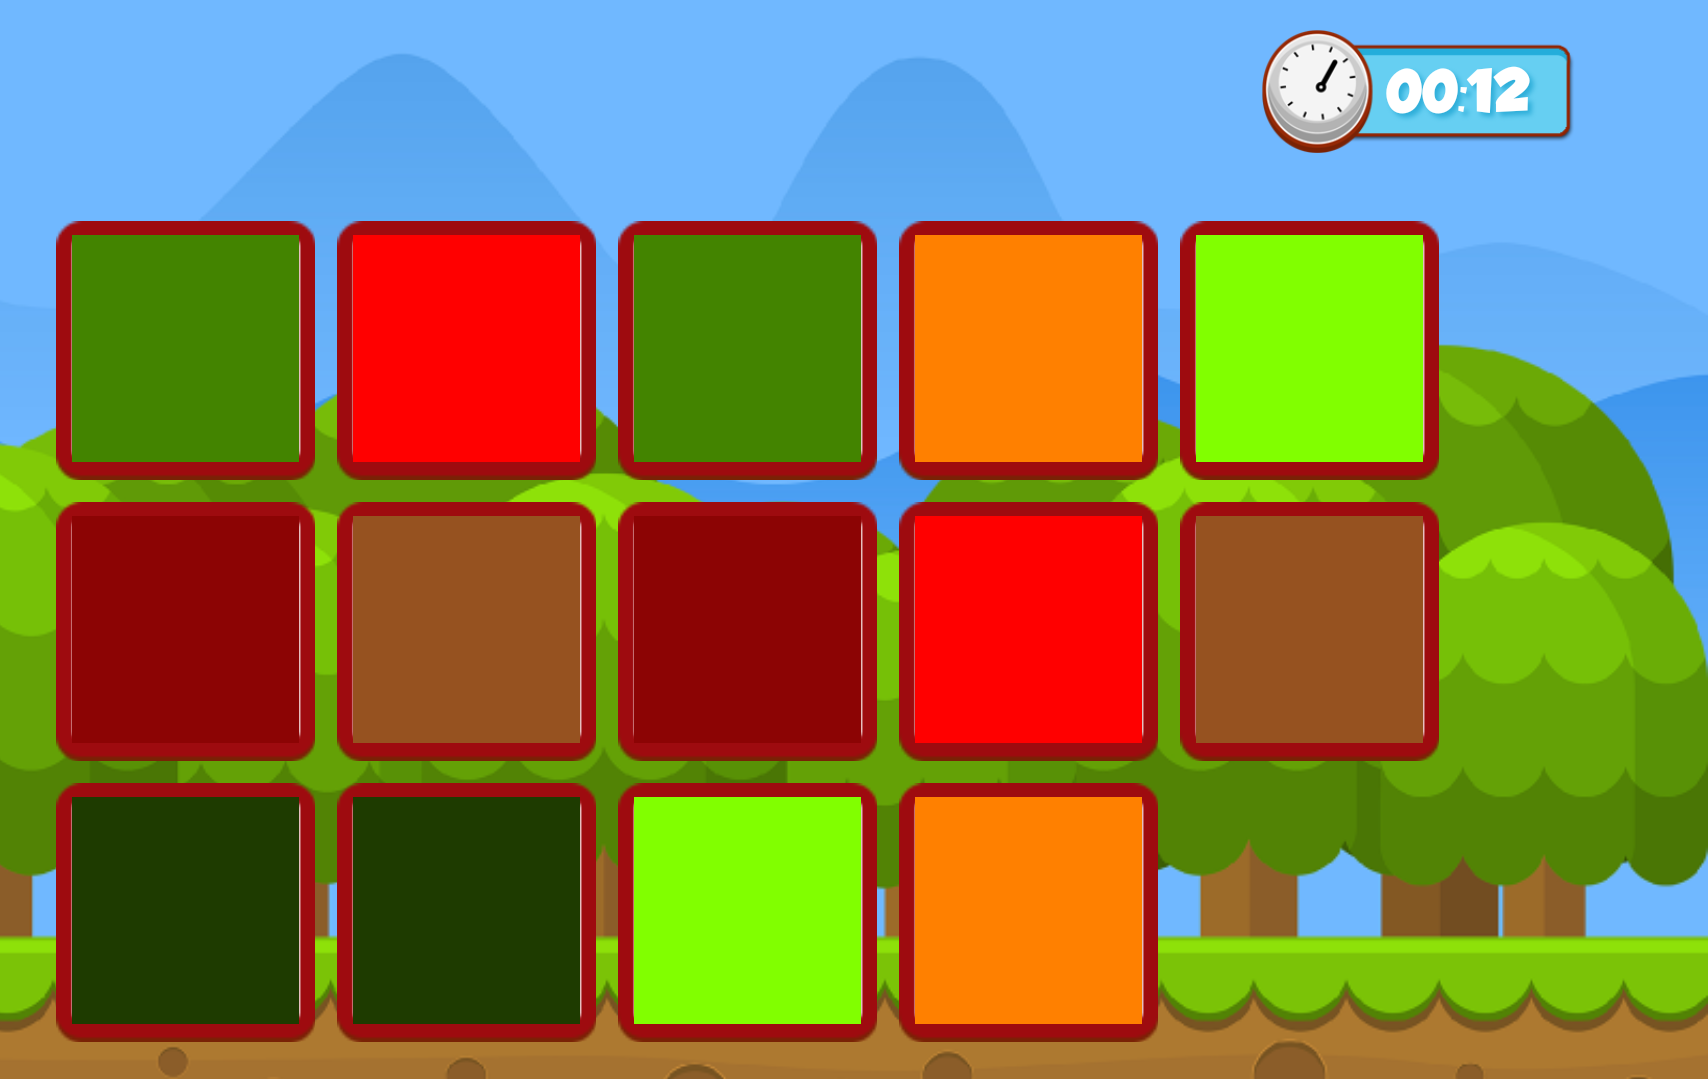
\includegraphics[width=14cm]{images/noObstTurned.png}
	\caption[Bild kurz]{Screenshot of the game without obstacles. All cards are turned face up.}
	\label{fig:noObstacle}
\end{figure}

\begin{figure}[H]
	\centering
	
\includegraphics[width=14cm]{images/glareEffect.png}
	\caption[Bild kurz]{Screenshot of the game field with simulated sunlight. Sunbeams are especially visible on the right hand side. All cards are turned face up.}
	\label{fig:glareEffect}
\end{figure}